% !TEX root = univariate.tex

UnivariePour commencer, ce rapport comportera une analyse univariée de chacune des variables quantitatives et qualitatives qui font partie de le jeu de données, en suite il passera a l'analyse bivariée pour vérifier des liens entre les variables quantitatives mesurées par la corrélation linéaire.

\begin{figure}
    \centering
    \subfloat[hits]{
        \label{hits}
        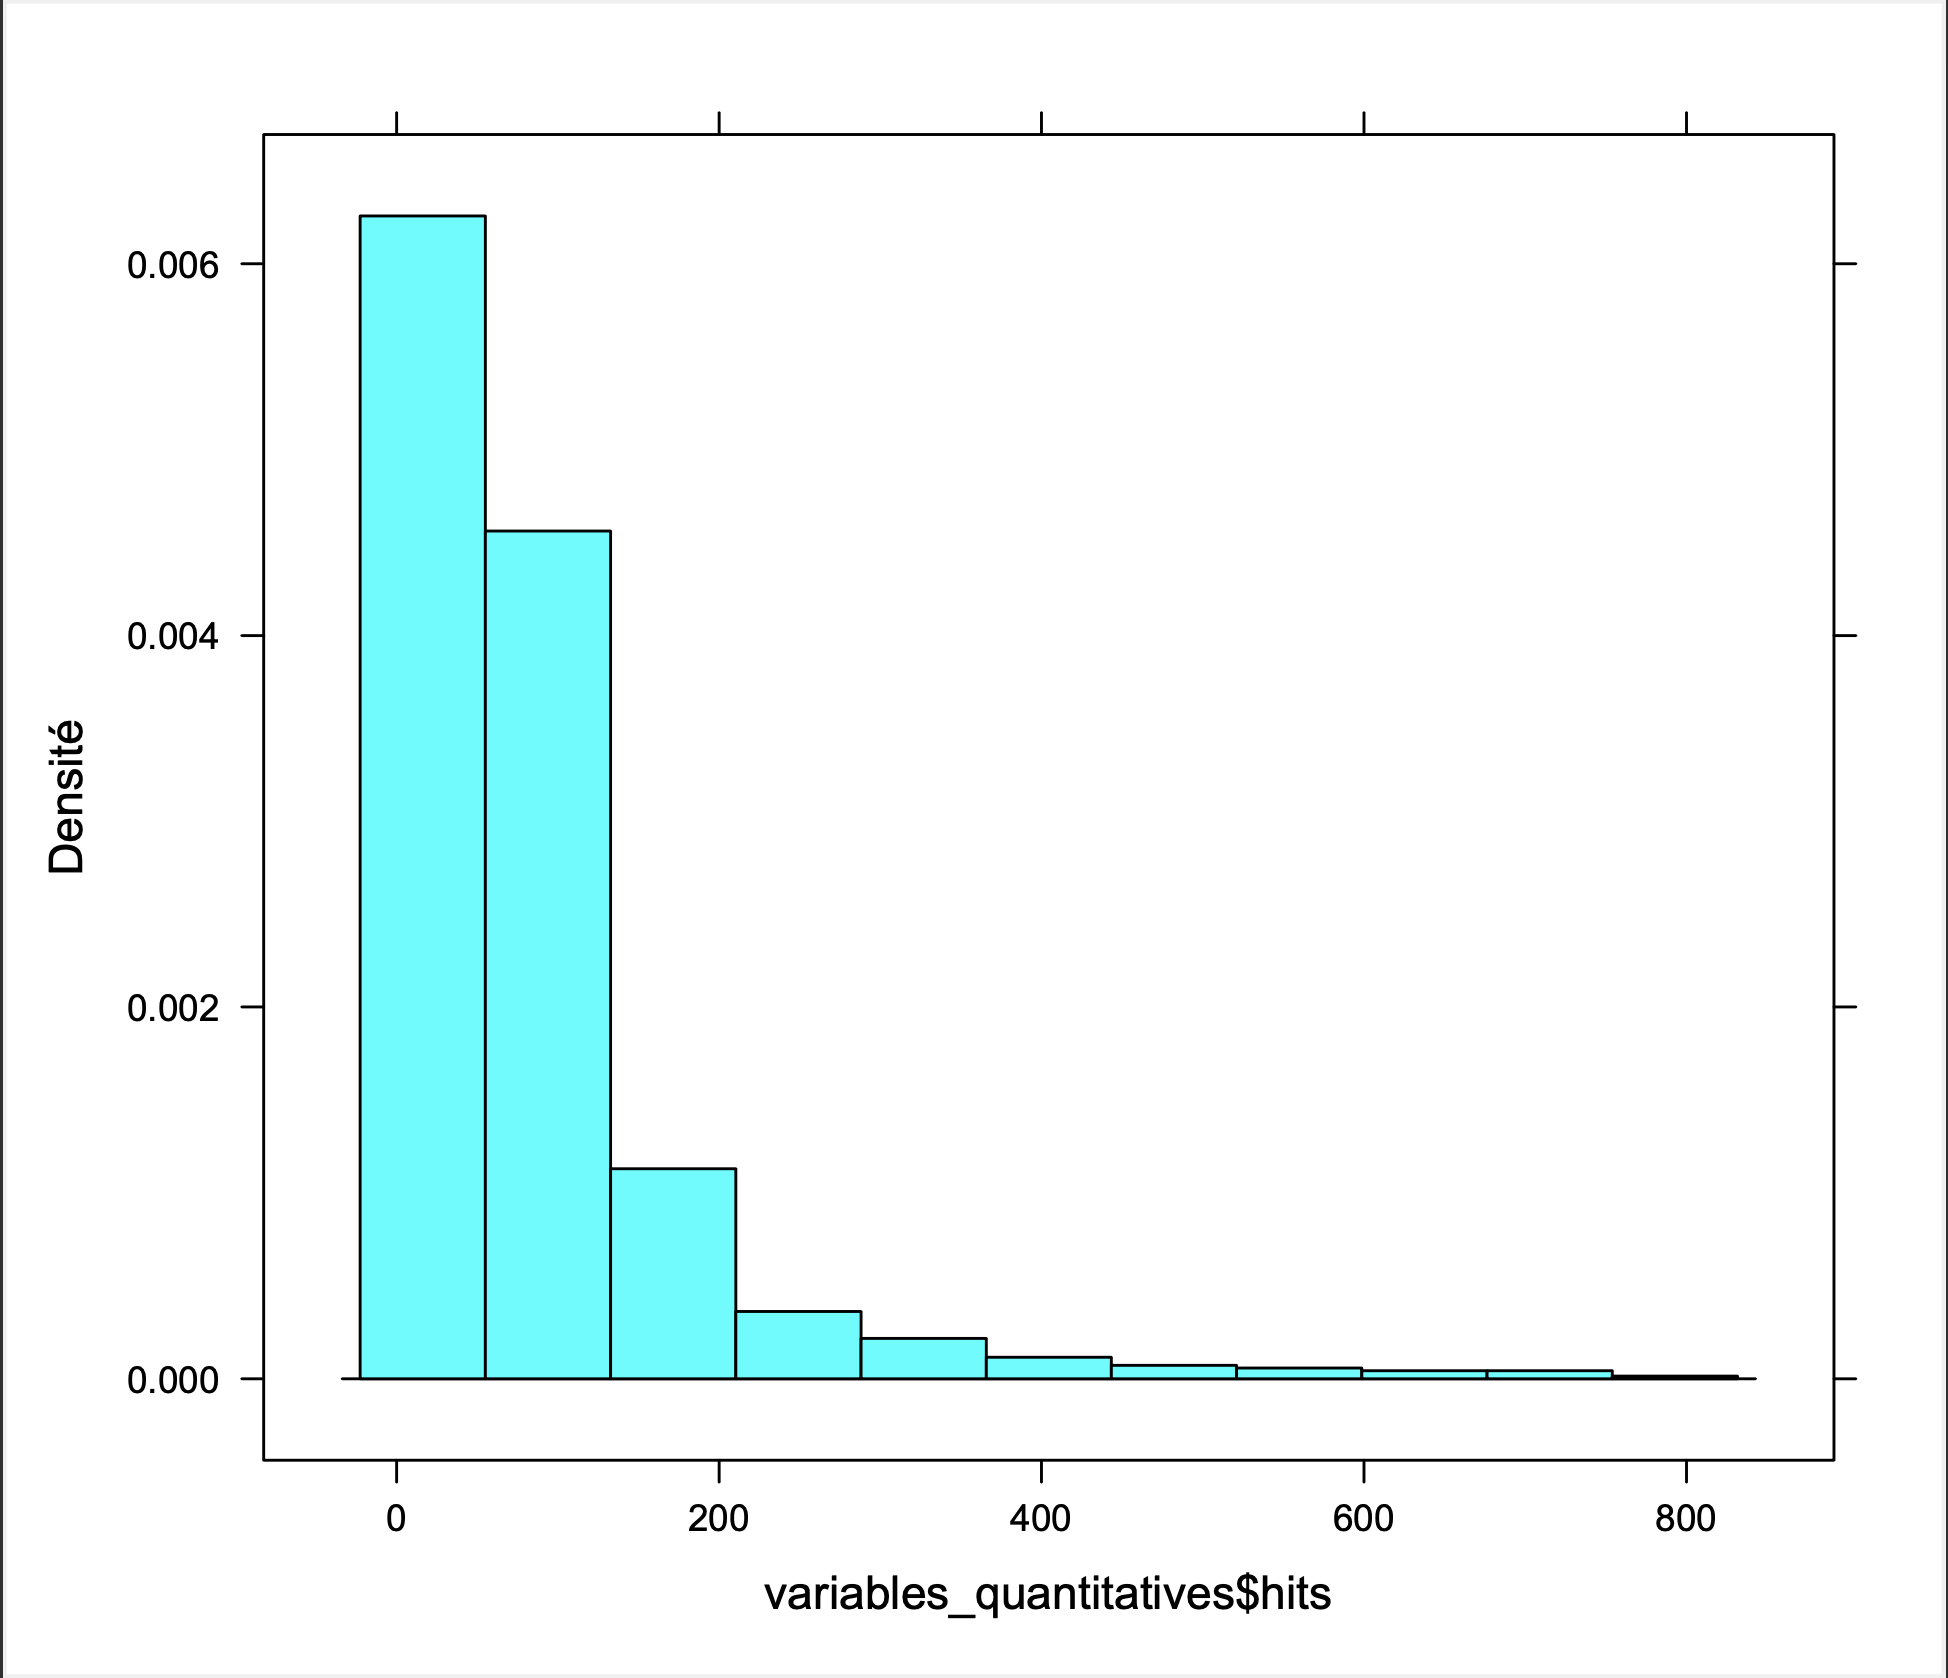
\includegraphics[width=0.45\textwidth]{scriptsR/imgs/univarie/hits.png}
    }
    \hfill
    \subfloat[New visit]{
        \label{new_visits}
        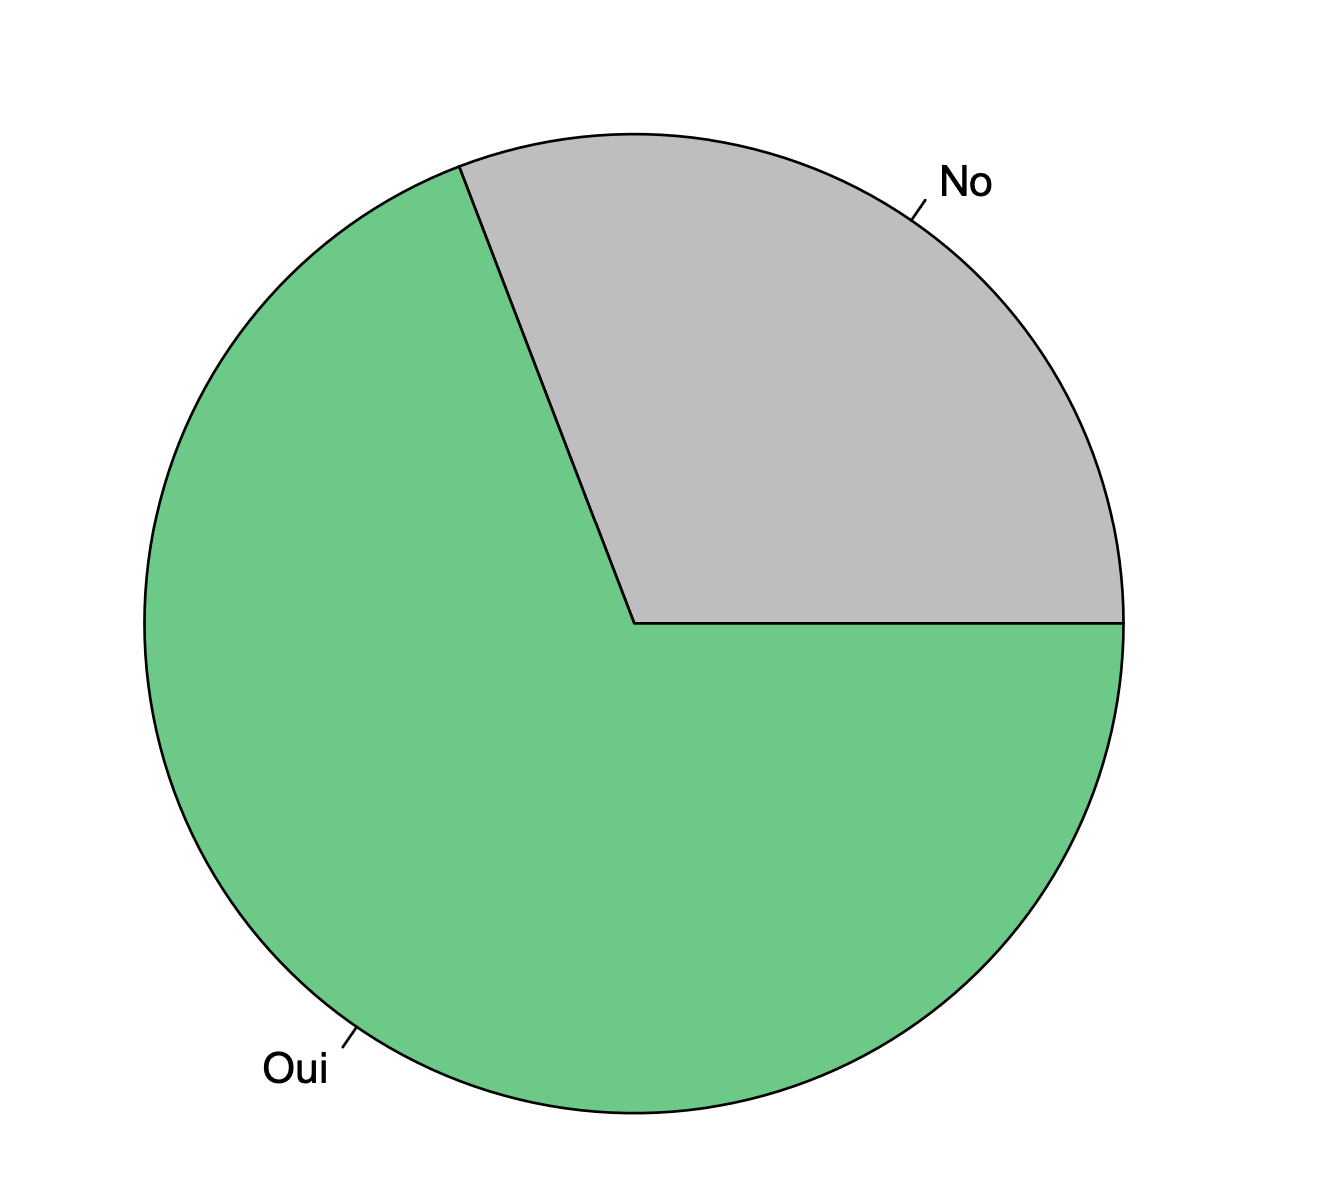
\includegraphics[width=0.45\textwidth]{scriptsR/imgs/univarie/newVisit.png}
    }
     \hfill
    \subfloat[Page views]{
        \label{page_views}
        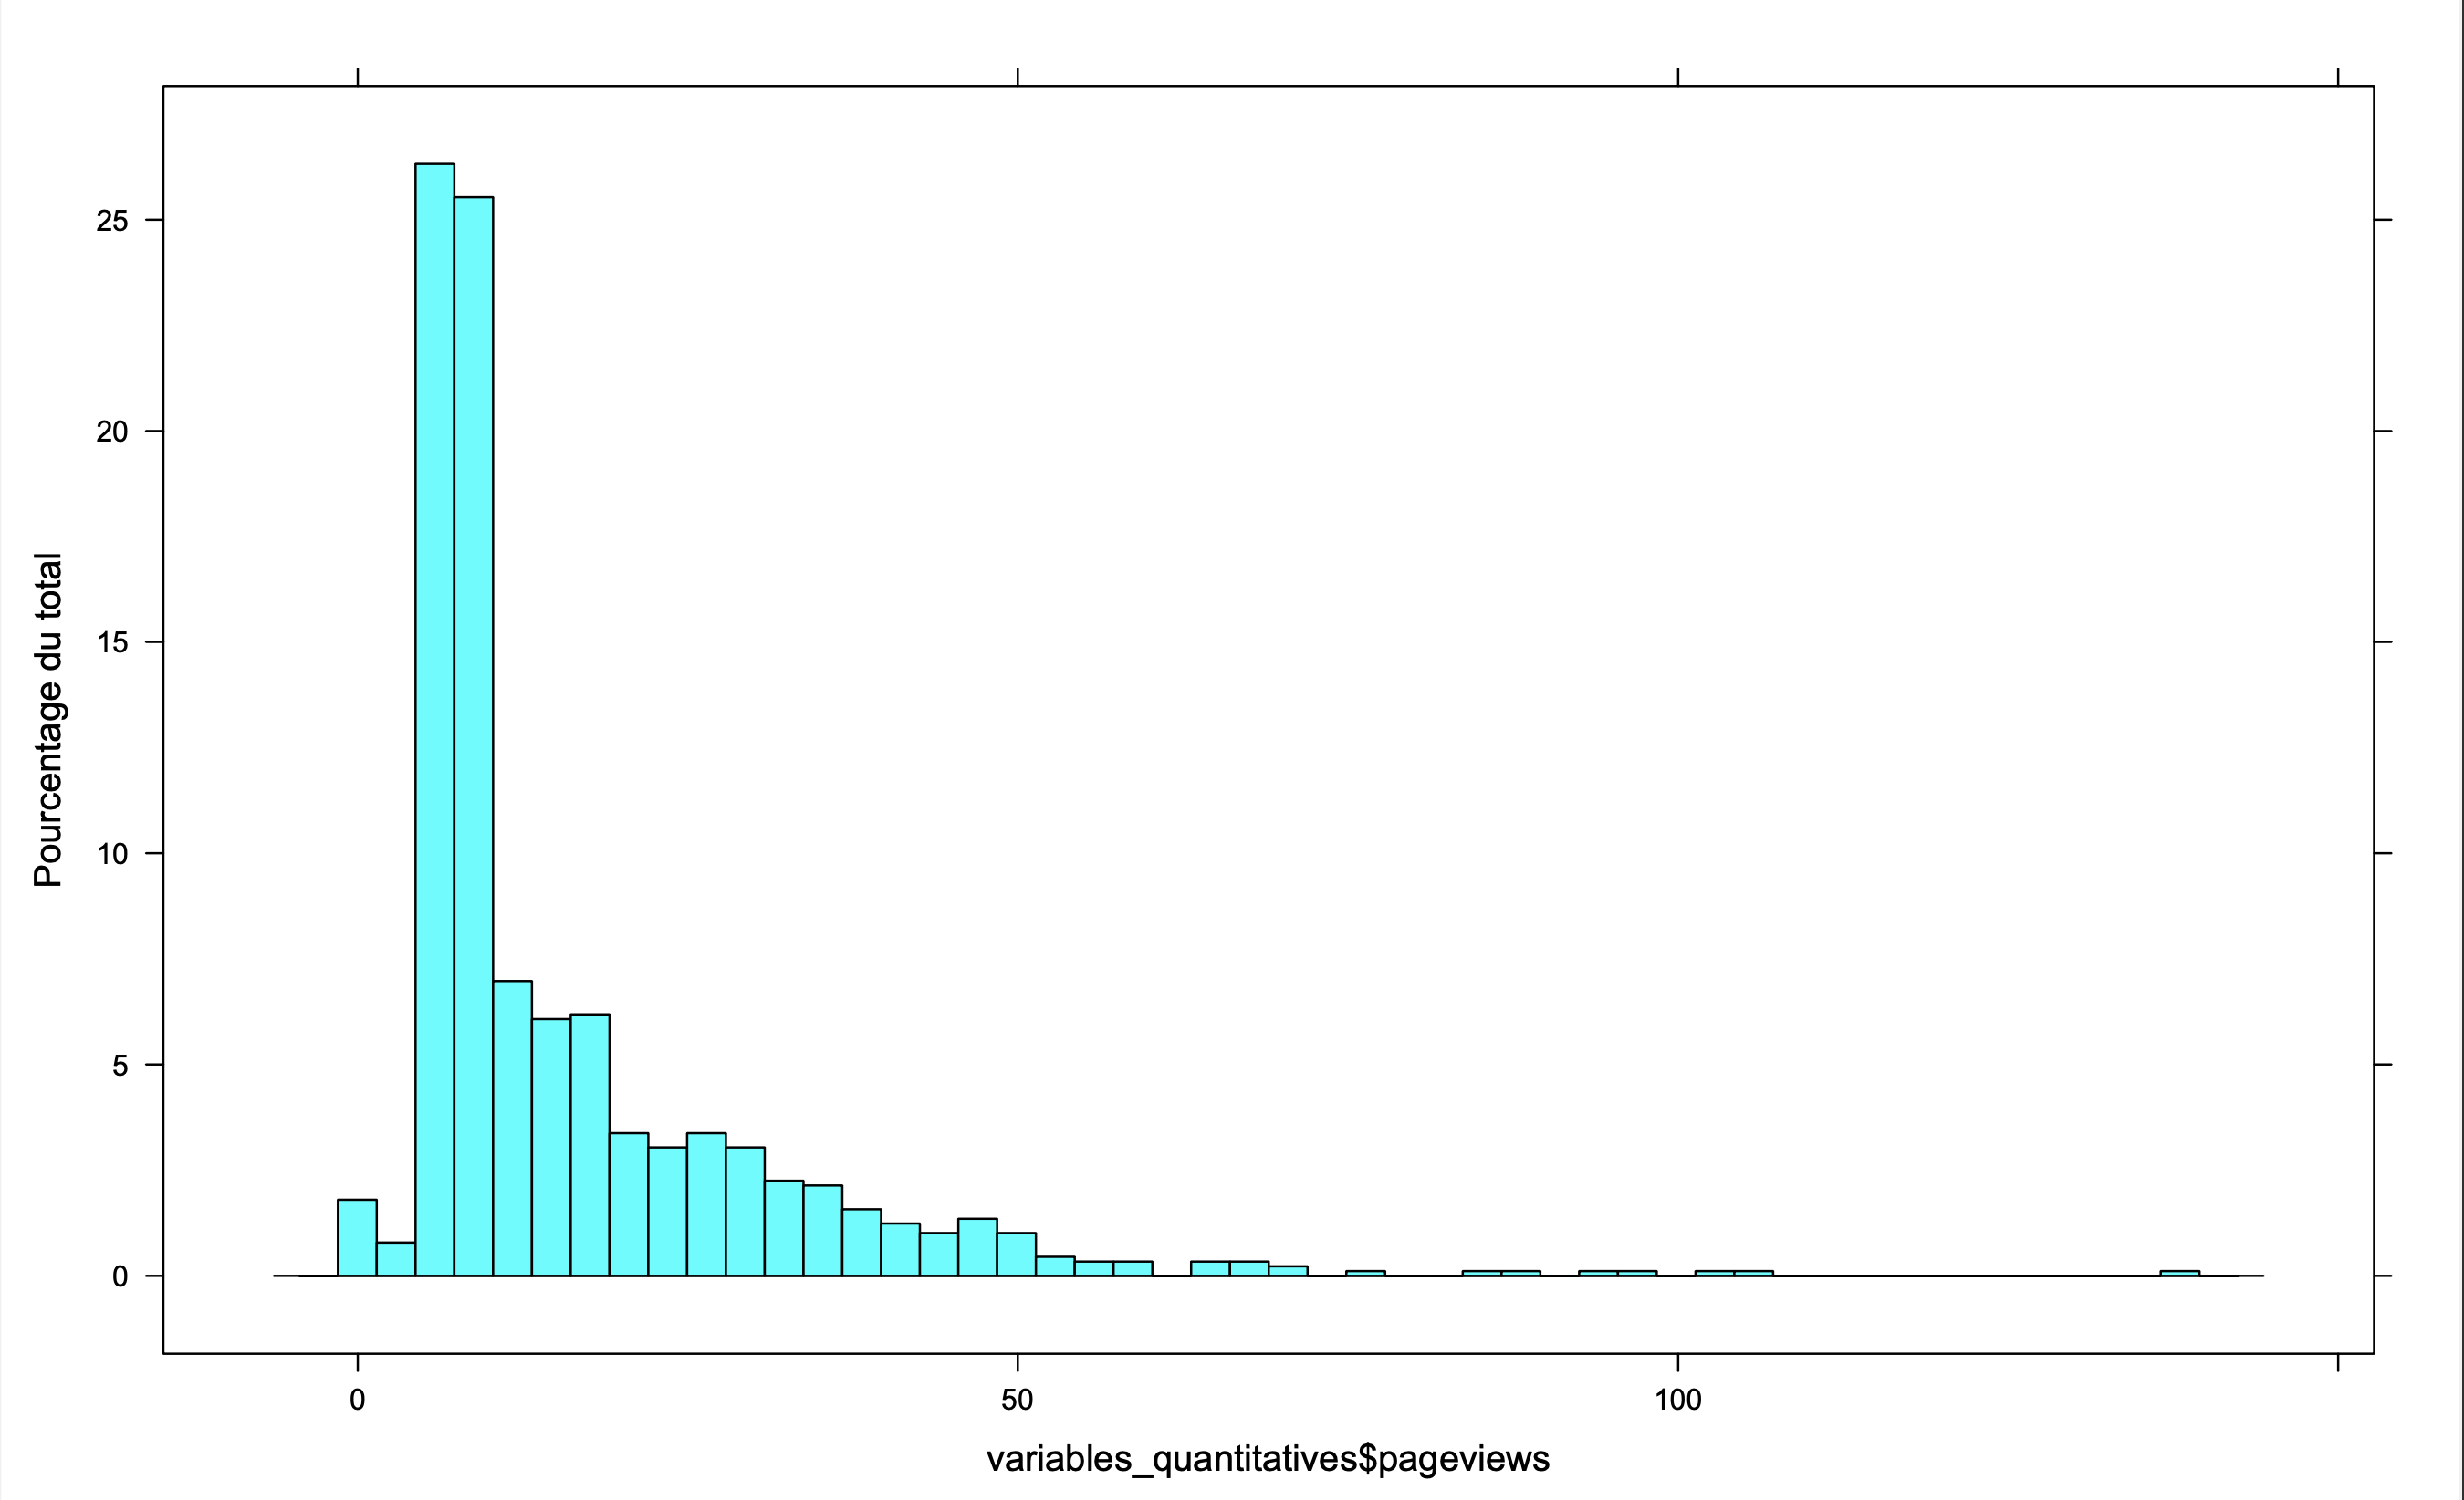
\includegraphics[width=0.45\textwidth]{scriptsR/imgs/univarie/page_views.png}
    }
    \hfill
    \subfloat[Total transaction revenue]{
        \label{transaction_revenue}
        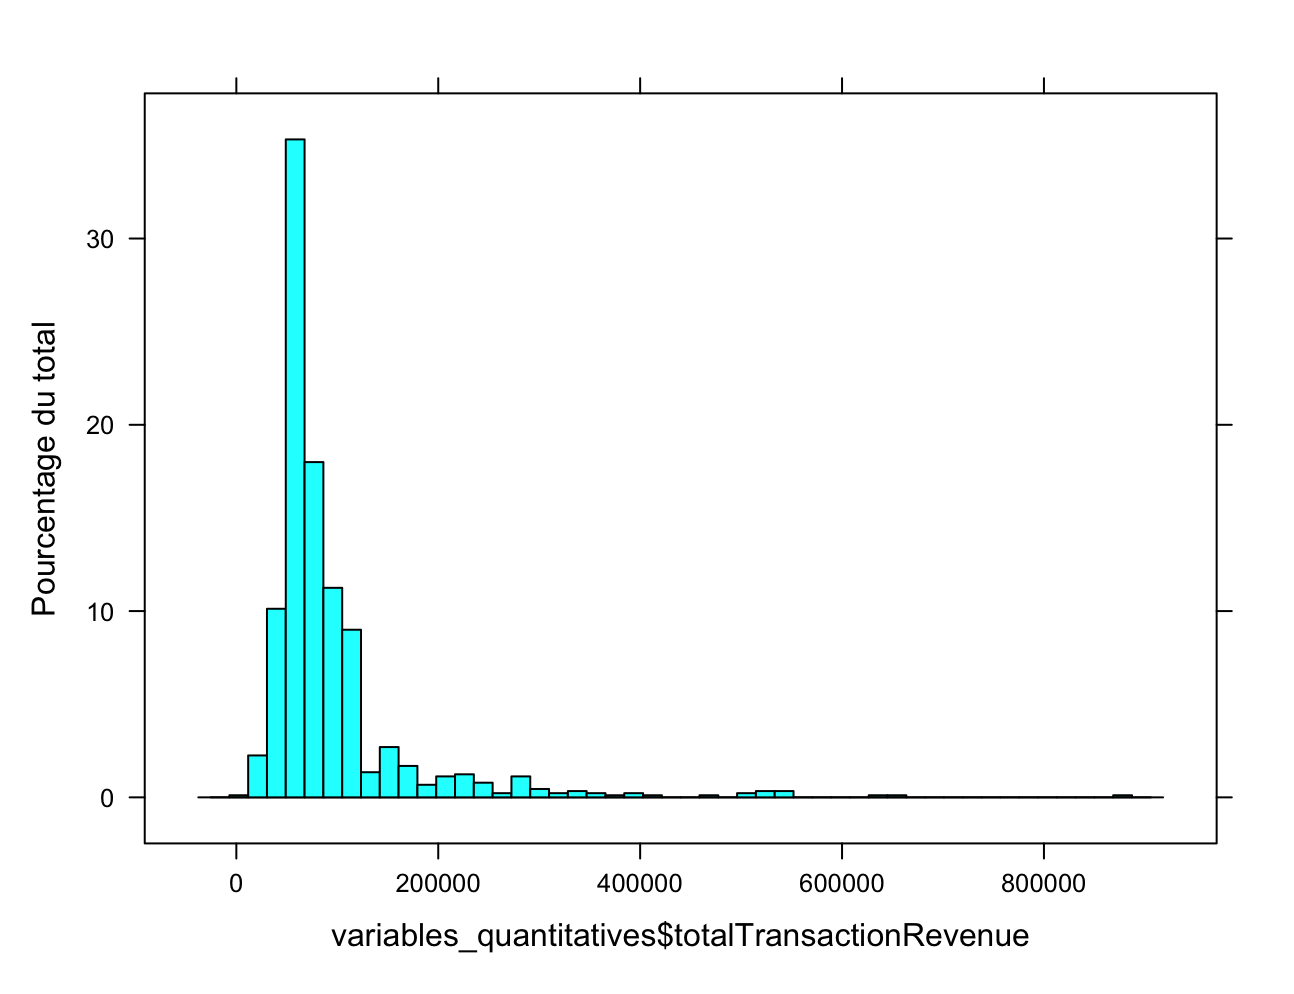
\includegraphics[width=0.45\textwidth]{scriptsR/imgs/univarie/TotalTransactionHistogram.png}
    }
    \caption{Overall caption}
    \label{ref_label_overall}
\end{figure}
